\documentclass[journal]{IEEEtran}
\usepackage{times}

% numbers option provides compact numerical references in the text. 
\usepackage[sort,compress,numbers]{natbib}
\usepackage{multicol}
\usepackage[bookmarks=true]{hyperref}
\usepackage{graphicx}
\usepackage{amsmath}
\usepackage{array}
\usepackage{algpseudocode}
 
% \usepackage{caption}
\usepackage{indentfirst}
\usepackage{amsmath}
\usepackage{multirow}
\usepackage{array}
\usepackage{algpseudocode}
\usepackage{epstopdf}
\newcommand{\rr}{\raggedright}
\newcommand{\tn}{\tabularnewline}
\newcommand{\shortcite}[1]{\cite{#1}}
\newcommand{\degree}{\ensuremath{^\circ}}


%\pdfinfo{
%   /Author (
%   % Omitted to meet double-blind review requirements % 
%   Lanny Lin and Michael A. Goodrich)
%   /Title  (Hierarchical Heuristic Search Using A Gaussian Mixture Model for UAV Coverage Planning)
%   /CreationDate (D:20130304120000)
%   /Subject (Algorithm Paper)
%   /Keywords (UAV, Path Planning, Coverage)
%}

\begin{document}

% paper title
\title{Sliding Autonomy for UAV Path Planning: Adding New Dimensions to Autonomy Management}

% You will get a Paper-ID when submitting a pdf file to the conference system
\author{
% Author Names Omitted for Anonymous Review. Paper-ID 158 %
Lanny~Lin,~\IEEEmembership{Member,~IEEE,}
and~Michael~A.~Goodrich,~\IEEEmembership{Senior~Member,~IEEE}%
\\Computer Science Department \\ Brigham Young University \\ lanny.lin@byu.edu, mike@cs.byu.edu
}

\maketitle

\begin{abstract}
Increased use of autonomy also increases human-autonomy interaction and the need for humans to manage autonomy. We propose a new autonomy management approach, sliding autonomy, where the user can influence the behavior of the autonomous system along three new dimensions: information representation, task constraints (spatial), and time allocation (temporal). We analyze how this approach fits in the integration challenges guideline we identified in our prior work and apply it to the task of UAV (Unmanned Aerial Vehicle) path planning to support Wilderness Search and Rescue (WiSAR). We evaluate the usefulness of the approach against manual and simple pattern path planning methods with a user study. Results show that the sliding autonomy approach performs significantly better than the other two methods without increasing the users' mental workload, and the performance of the human-autonomy team outperforms either human or autonomy working alone. We also discuss some interesting observations from the user study.
\end{abstract}


\begin{IEEEkeywords}
Unmanned aerial vehicles, path planning, navigation, adjustable autonomy, supervisory control
\end{IEEEkeywords}

\IEEEpeerreviewmaketitle


%=================================================================================
\section{Introduction}
\label{sec:Introduction6}

% First talk about need for autonomy management, especially for domain experts who don't know or care about how autonomy works
\IEEEPARstart{W}{ith} the rapid advancement in technology, people are seeing increased use of autonomy to augment human abilities and support human decision-making in many application domains (e.g.,~\cite{Chun2010Limousine,Casper2003Human,Lin2010Supporting,Robins2009From}). At the same time, increased use of autonomy also means increased human-autonomy interaction and increased need for human to manage autonomy~\cite{Bainbridge1983Ironies}. Even for fully autonomous systems, human input can potentially improve the system's performance and safety. The managerial responsibilities include monitoring the safety of the autonomous system, supervising autonomy to achieve acceptable performance, and making sure autonomy is working toward the collective goal of the overall system. The human operators are domain experts who can use domain-specific knowledge to assist the autonomous system when it deals with changing environments, uncertainty, and case-specific scenarios. However, the humans in such interactions are not likely the designers of the autonomous systems, but these humans must still manage autonomy, because ``only people are held responsible for consequences (that is, only people can act as problem holders) and only people decide on how authority is delegated to automata''~\cite{Woods2006Joint,Bradshaw2013Seven}. Therefore, it is necessary to design tools and interfaces that enable human users to manage the autonomous behaviors of the system efficiently and effectively; such tools can improve task performance and the experience of the human operator in human-autonomy interaction.

% Then we describe our approach.
We propose a new autonomy management approach where the user can influence the behavior of the autonomous system along three new dimensions: 1) \textbf{Information Representation}: user can modify information representation relate to the problem that autonomy can understand, such as areas of focus and task-difficulty; 2) \textbf{Task Constraints}: user can choose where to add constraints to the problem to change its properties; and 3) \textbf{Time Allocation}: user can decide how much time to allocate to a subtask out of the total task time. Once the information representation and task constraints are set, the user can move a slider to control how much time is allocated to the subtask and see immediately how the action affects the solution generated by autonomy. This is why we named our approach \textbf{Sliding Autonomy}. Full solution to the problem is combined from solutions of all the subtasks. It is most likely different from a solution generated by full autonomy because of the additional human-autonomy interaction. Ideally, humans should be doing what humans are good at, and autonomy should be doing what autonomy is good at (in reality, autonomy is also doing what humans do not want to do). The human-autonomy team should perform better than human or autonomy working alone.

% Briefly talk about existing approaches and what we propose, and why different.
Many approaches to autonomy management already exist, such as \textit{Supervisory Control}~\cite{Sheridan1992Telerobotics}, \textit{Mixed-initiative}~\cite{Hearst1999Mixed}, \textit{Collaborative Control}~\cite{Fong1999Collaborative}, \textit{Adjustable Autonomy}~\cite{Dorais1998AdjustableAutonomy,Dorais2001Designing} (also referred to as \textit{Sliding Autonomy}~\cite{Dias2008SlidingAutonomy} or \textit{Adaptive Automation}~\cite{Rouse1988Adaptive,Kaber2001Design}). The approach we propose falls under the category of \textit{Adjustable Autonomy}. The three dimensions we identified are in addition to dimensions of \textit{Adjustable Autonomy} identified by Bradshaw et al.\ in~\cite{Bradshaw2004Dimensions}.

% Talk about that we extended our guideline
In our previous work~\cite{Lin2010Supporting} we identified key elements of autonomy integration challenges along two dimensions: \textit{attributes of an intelligent system} (capability, information management, performance evaluation) and \textit{scale} (individual versus group), which can serve as a guideline in designing autonomous components and autonomy management tools. In this paper we extend this guideline to include attributes needed when human and autonomy work collaboratively. We apply the proposed approach to the task of UAV (Unmanned Aerial Vehicle) path planning to support Wilderness Search and Rescue (WiSAR), describe what these three new dimensions mean in this context, and explain how they fit in the guideline we defined.

% Discuss what application domain we apply this to, and the benefits.
Camera-equipped mini-UAVs can be useful tools in WiSAR operations by providing aerial imagery of a search area with the benefits of quick coverage of large areas, access of hard-to-reach areas, and lower cost than manned aircraft~\cite{Murphy2008Cooperative, Goodrich2008Supporting}. In fact Canadian mounties claim that they have successfully saved a person with a police drone in a recent rescue mission\footnote{http://www.theverge.com/2013/5/10/4318770/canada-draganflyer-drone-claims-first-life-saved-search-rescue}. UAV path planning is an important task because a good flight path can increase the probability of finding a missing person by making efficient use of the limited flying time. Various algorithms have been developed to generate UAV paths automatically (e.g.,~\cite{Bourgault2003Coordinated, Lin2009UAV, Lin2014Hierarchical}). By applying sliding autonomy to this path planning task, we argue that this approach:
\begin{itemize}
\item enables the domain expert user to incorporate information only available to or understandable by the user;
\item is easy to understand without knowing how autonomy works behind the scene;
\item lets the human do what human is good at (planning strategically) and autonomy do what autonomy is good at (planning tactically), resulting in better performance than human or autonomy working alone;
\item enables the user to align task goal with system goal;
\item and improves human's experience during the human-autonomy interaction.
\end{itemize}

% We did user study to evaluate the approach. What are the results.
To evaluate the usefulness of the proposed approach, we performed a user study and compared the sliding autonomy method against two other planning methods (manual and simple pattern path planning) in two WiSAR scenarios (a synthetic scenario and a real scenario). We measured each user's performance with each method and also the user's performance on a secondary task (answer questions in a group chat window). Experiment results show that the sliding autonomy method performed significantly better than the manual or simple pattern planning methods with no increased mental workload. The human-autonomy team also performed better than the human or autonomy working alone.

% What does each section talk about?
In section~\ref{sec:dimensions} we explain how the proposed approach fits into the extended autonomy design guideline and describe how a user can manage autonomy along each of the three new dimensions in the context of UAV path planning. Section~\ref{sec:RelatedWork6} covers related work in literature. Section~\ref{sec:Hypotheses} lists our hypotheses followed by user study design in section~\ref{sec:Design}. Then we present experiment results in section~\ref{sec:Results} and discuss our observations in section~\ref{sec:Discussion}. In section~\ref{sec:Conclusions6} we conclude the paper and list possible future work.

\begin{figure}
\centering
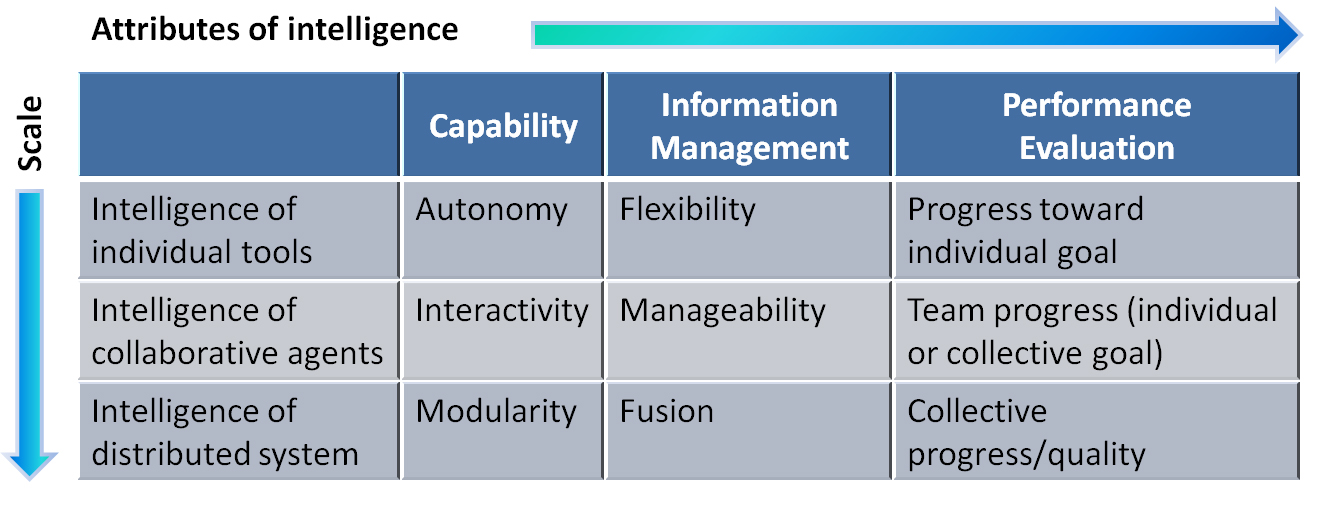
\includegraphics[width=3.5in]{IntegrationChallenges.JPG}
\caption{Autonomy integration challenges defined along two dimensions. Horizontal dimension: attributes of intelligence. Vertical dimension: scale.}
\label{IChallenges}
\end{figure}

%=================================================================================
\section{Autonomy Design Guideline and New Dimensions}
\label{sec:dimensions}

%===================================================
\subsection{Autonomy Design Guideline}

In our previous work~\cite{Lin2010Supporting} we organized the challenges of autonomy and management tool design along two dimensions: \textit{attributes of an intelligent system} (capability, information management, performance evaluation) and \textit{scale} (individual versus group), which can serve as a guideline in designing autonomous components and autonomy management tools. Here we extend this table by adding a row in the middle describing what attributes are needed when multiple agents work collaboratively (see Figure~\ref{IChallenges}). A human-autonomy team working on the same task falls within this category. As an individual tool, an autonomous component needs to be able to perform a task (\textbf{Autonomy}); the operator can match capability to task according to the information available to the operator, which requires that autonomy can be interrupted, paused, aborted, and resumed (\textbf{Flexibility}); the performance is evaluated to match individual task goal. When a human-autonomy team works on the same task collaboratively, the autonomous component needs to provide interfaces so the human can influence the autonomous behavior with human inputs (\textbf{Interactivity}); the human agent should be able to manage how autonomy works in order to jointly find a solution by utilizing information only available to the human agent and/or feed information to autonomy in a representation that autonomy can understand (\textbf{Manageability}); and when performance is evaluated, the human operator can judge whether the individual goal aligns with the collective goal of the system. As part of a larger distributed system, each autonomous component needs to be modular (\textbf{Modularity}), so they can be mixed and matched to support different user roles; information from various sources need to be combined and presented to one or multiple users in a \textbf{Fusion}; and performance of the system needs to be evaluated as a whole. This paper focuses on the middle row of this guideline: intelligence of collaborative agents (human-autonomy team). The three dimensions we propose are ways path planning autonomy can be managed, and the path planner component is designed to accept human inputs along the three dimensions to provide interactivity. The human can also incorporate information from various sources and influence the behavior of path planning autonomy, making sure the task goal aligns with the ultimate goal of finding the missing person quickly.

\begin{figure}
\centering
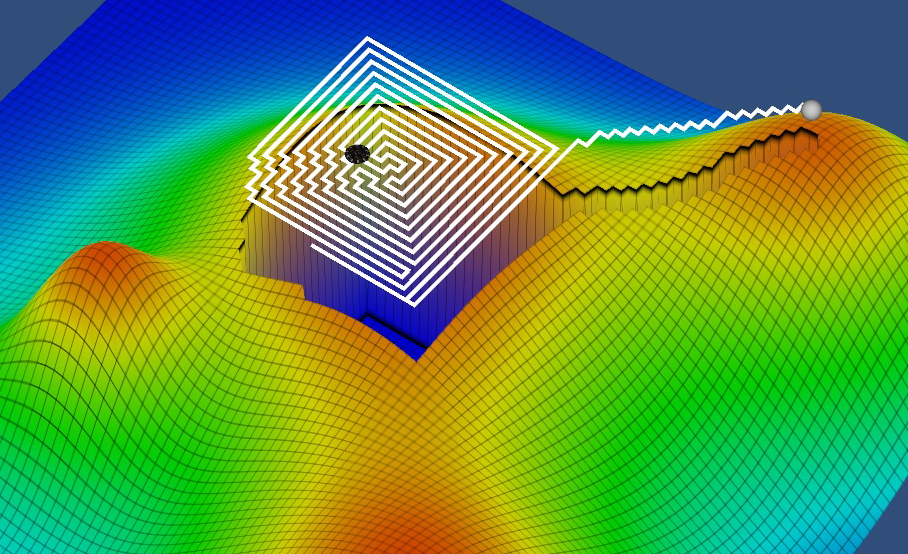
\includegraphics[width=3.5in]{Dimensions.JPG}
\caption{A screen capture of the sliding autonomy tool showing a 20 minute path. The 3D surface shows the probability distribution map. The UAV icon in the middle indicates the start point of the path segment and the sphere on the right indicate the end point.}
\label{dimensions}
\end{figure}

%===================================================
\subsection{Information Representation Dimension}

Many path planning algorithms use a probability distribution map that shows where are likely places to find the missing person. We also designed our path planning algorithms to support a task-difficulty map: a spatial representation showing (one minus) sensor detection probability in different parts of the search region. For example, probability near the last known position (LKP) of the missing person is normally high (low task difficulty); and the probability of detecting the missing person in a dense vegetation area from camera footprints is normally low (high task difficulty). The objective of path planning is to find a path that maximize the detection probability of the missing person given a fixed flying time. The maps can be systematically generated based on terrain features and vegetation data~\cite{Lin2010Bayesian, Lin2014Hierarchical}. However, the searcher likely wants to include his/her domain expertise (past experience, knowledge of the search region, etc.) and additional information (maybe new evidence found during the search) in the planning. These types of information are not directly understandable by autonomous algorithms, but the searcher can incorporate them into the probability distribution map and the task-difficulty map using map editing tools\footnote{Such as these tools at http://tech.lannyland.com/demos.html.}, thus influence the behavior of path planning autonomy. Marking an area with high probability, the searcher indirectly tells the UAV to treat the area with high priority; marking an area with high task-difficulty, the UAV might make multiple passes over the area to search more thoroughly. The 3D surface in Figure~\ref{dimensions} shows an example probability distribution map where hills (red) indicate high probability and the flat area (blue) indicates low probability.

By managing information representation, the searcher can quickly figure out how his actions will affect the behavior of autonomy, even though he/she has no idea about how autonomy works behind the scene. Our interface supports autonomy management along this dimension. But we choose to not include it in the current user study (due to the one-hour limit per test subject) and leave the evaluation in a separate user study.

%===================================================
\subsection{Task Constraints Dimension}

The searcher can also influence the behavior of path planning autonomy by adding constraints to the problem. Constraints can be the start/end points of the path or no-fly zones. Setting an end point in an area is a way for the searcher to indirectly tell path planning autonomy that he/she wants the UAV to search this area. For example, if a piece of clothing is found by the ground team, the searcher can force path planning autonomy to go visit that area by setting an end point there. The searcher can also use this method to direct path planning autonomy to not visit an area (maybe the area has been thoroughly searched by the ground team) by setting the end point in other areas. By managing autonomy along this dimension, the searcher can incorporate additional information, information not directly understandable by autonomy, to improve task performance and align the task goal with the overall goal of finding the missing person quickly. A no-fly zone is pretty straight forward way to restrict the UAV from visiting certain areas maybe due to safety reasons. In Figure~\ref{dimensions}, the UAV icon in the middle indicates the start point of the path segment and the sphere on the right side indicates the desired end point. Because start/end points and no-fly zones are all spatial constraints, the searcher manages autonomy along a spatial dimension.

Spatial constraints are easy to understand, so the searcher knows how these constraints will affect the behavior of path planning autonomy. In our user study we fixed the start point of the path to the center of the map because that was the last know position of the missing person. The searcher can set the end point for the current path segment anywhere on the map, and this end point automatically becomes the start point for the next path segment. No-fly zone was not included in this user study (it was tested in a separate user study~\cite{Clark2013Hierarchical}).

%===================================================
\subsection{Time Allocation Dimension}

Once the information representation and task constraints (optional) are set, the searcher can use a slider to allocate different time to path planning autonomy. For example, as shown in Figure~\ref{dimensions}, for a 60-minute total flight, the searcher can set an end point to the probability hill on the right, and then move the slider to see immediately what path segment autonomy would suggest. The path segment shown is when 20 minutes are allocated. If the searcher is happy with the suggestion, he approves the path segment. The UAV moves to the end point and ``vacuums up'' the probability along the path (how much can be vacuumed up is determined by the task-difficulty map). Then the searcher works together with autonomy to plan the path for the remaining 40 minutes. The two (or more) path segments are joined to form the final path. In the example shown, the combination of the information representation, task constraints, and time allocation allows the searcher to cover the middle area pretty well and then move to the search area on the right ready to search there. If no constraint is set, autonomy might decide to search the probability hill on the left instead. If more flight time is allocated with the set end point, autonomy might start searching the area on the right. Because the searcher decides how many path segments to plan and how much time to allocate to each path segment, the searcher manages autonomy along a temporal dimension.

As the searcher moves the slider to control time allocation, the sliding autonomy tool provides suggested path segment immediately. This instant feedback provides the searcher the ability to perform ``what-if'' analysis and see the causal effect between his/her action and changes in autonomous behavior. 

By managing time allocation, the searcher can break the path planning task into subtasks. The objective of path planning autonomy is to maximize the amount of probability the UAV can collect following the current path segment. The objective of the human or the entire distributed system (where the UAV is only a part of the operation) is to find the missing person quickly. By setting constraints and change the amount of time allocated to a path segment, the searcher has the ability to incorporate additional information into the problem, and align the task goal with the overall system goal. The ability to break the task into subtasks also enables the searcher to plan more strategically (prioritizing areas in the entire search region) while autonomy works more tactically (covering the current search area well). Ideally such a human-autonomy team should work better than either human or autonomy working alone.


%=================================================================================
\section{Related Work}
\label{sec:RelatedWork6}

Drucker defines automation as a ``concept of the organization of work~\cite{Drucker2006Practice}.'' Goodrich and Schultz~\cite{Goodrich2007HRISurvey} define the HRI problem as ``understanding and shaping the interactions between one or more humans and one or more robots.'' They also specified robot-assisted search and rescue as a key area for HRI research. In their 1978 seminal paper~\cite{Sheridan1978Human}, Sheridan and Verplank propose the idea of a \textit{Level of Autonomy} spectrum, with full teleoperation at one end and full autonomy at the other. In the middle, the robot could suggest actions to humans or make decisions before informing humans. Parasuraman et al.\ \cite{Parasuraman2000Model} extended this one-dimensional spectrum to four different broad functions: information acquisition, analysis, decision selection, and action implementation. In~\cite{Sheridan1992Telerobotics} Sheridan proposes \textit{Supervisory Control}, in which a human divides the task into a sequence of subtasks that the robot is capable of performing, and the human then provides guidance when the autonomous system cannot solve a problem on its own. In contrast to the top-down philosophy of supervisory control, a \textit{Mixed-initiative} approach advocates the idea of dynamically shifting tasks when necessary~\cite{Hearst1999Mixed}. \textit{Collaborative Control}, which can be thought of as an instance of mixed-initiative interaction, is a robot-centric model; instead of the human always being in-charge, the robot is treated as a peer and can make requests to humans through dialogs~\cite{Fong1999Collaborative}. \textit{Adjustable Autonomy}~\cite{Dorais2001Designing} (also referred to as \textit{Sliding Autonomy}~\cite{Dias2008SlidingAutonomy} or \textit{Adaptive Automation}~\cite{Rouse1988Adaptive}) is another type of mixed-initiative interaction, one that enables the human-automation team to dynamically and adaptively allocate functions and tasks among team members. 

Dorais et al.\ \cite{Dorais1998AdjustableAutonomy} discuss a framework for human-centered autonomous systems for a manned Mars mission. The system enables users to interact with these systems at an appropriate level of control but minimize the necessity for such interaction. Bradshaw et al.\ discuss principles and pitfalls of adjustable autonomy and human-centered teamwork, and then present study results on so-called ``work practice modeling'' and human-agent collaboration in space applications~\cite{Bradshaw2003AdjustableAutonomy}. In~\cite{Kaber2005Adaptive} Kaber et al.\ describe an experiment simulating an air traffic control task where manual control was compared to Adaptive Automation (AA). Results suggest that humans perform better with AA applied to sensory and psychomotor information-processing functions than with AA applied to cognitive functions; these results also suggest that AA is superior to completely manual control. Brookshire et al.\ present preliminary results for applying sliding autonomy to a team of robots performing coordinated assembling work to help the system recover from unexpected errors and to thereby increase system efficiency~\cite{Brookshire2004Preliminary}. Dias et al.\ identified six key capabilities that are essential for overcoming challenges in enabling sliding autonomy in peer-to-peer human-robot teams~\cite{Dias2008SlidingAutonomy}. Bradshaw et al.\ \cite{Bradshaw2004Dimensions} propose two dimensions of Adjustable Autonomy (descriptive and prescriptive) to address the two senses of autonomy (self-sufficiency and self-directedness) and discuss how permissions, obligations, possibilities, and capabilities can be adjusted. Bradshaw et al.\ \cite{Bradshaw2013Seven} also summarized some widespread misconceptions on autonomy and listed seven deadly myths of ``autonomous systems.''

Human is an integral part of the human-autonomy team. When working with autonomy, the human often takes on the supervisor role. Bainbridge points out that automation requires the human operator to take additional management responsibilities~\cite{Bainbridge1983Ironies}, and Sartar identified in~\cite{Sarter1998Making} two automation management policies: \textit{management by consent} and \textit{management by exception}, defining whether the human always retain authority or can the system take initiative. For complex automations, the human tends to rely on his/her \textit{mental models} (defined by Norman in~\cite{Norman1983Some}) to manage the system. 

UAV technology has emerged as a promising tool in supporting WiSAR~\cite{Murphy2008Cooperative,Bourgault2003Coordinated}. The goal of our research is to support fielded missions in the spirit of Murphy's work~\cite{Casper2003Human}. Many path planning algorithms in the literature address obstacle avoidance while planning a path to reach a destination using A*~\cite{Quigley2005Towards}, LRTA*~\cite{Howlett2006Learning}, D*~\cite{Stentz1997Optimal}, Voroni diagrams~\cite{Bortoff2000Path,Beard2005Autonomous}, or probability roadmaps and rapidly-exploring random tree (RRTs)~\cite{Pettersson2006Probabilistic}. Hierarchical heuristics approaches were also developed, such as Hierarchical A* (HA*) by Holte et al.\ ~\cite{Holte1996Hierarchical}, hierarchical task-based real-time path planning by Naveed et al.\ ~\cite{Meuleau2007Hierarchical}, and Hierarchical-AO* (HiAO*) by Meuleau and Brafman~\cite{Naveed2010Hierarchical}. In~\cite{Bourgault2006Optimal, Bourgault2004Coordinated} Bourgault et al.\ describe how to use a Bayesian model to create paths for a single UAV or multiple coordinated UAVs to maximize the amount of probability accumulated by the UAV sensors. The algorithms we used in this paper are algorithms designed from our previous work~\cite{Lin2009UAV,Lin2014Hierarchical} using techniques such as global warming technique, convolution, Gaussian mixture models, and Evolutionary Algorithm.

%=================================================================================	
\section{Hypotheses} 
\label{sec:Hypotheses}

We performed a user study to evaluate the usefulness with our proposed sliding autonomy approach. More specifically we verify the following hypotheses:

H1: Sliding autonomy method performs better than either the manual path planning method or a semi-autonomous simple pattern path planning method in both low information and high information scenarios.

H2: Sliding autonomy method performs better than autonomy working alone in both low information and high information scenarios.

H3: Sliding autonomy method does not increase the mental workload of the operator when compared against manual and pattern methods.

%=================================================================================	
\section{User Study Design} 
\label{sec:Design}

\begin{figure}
\centering
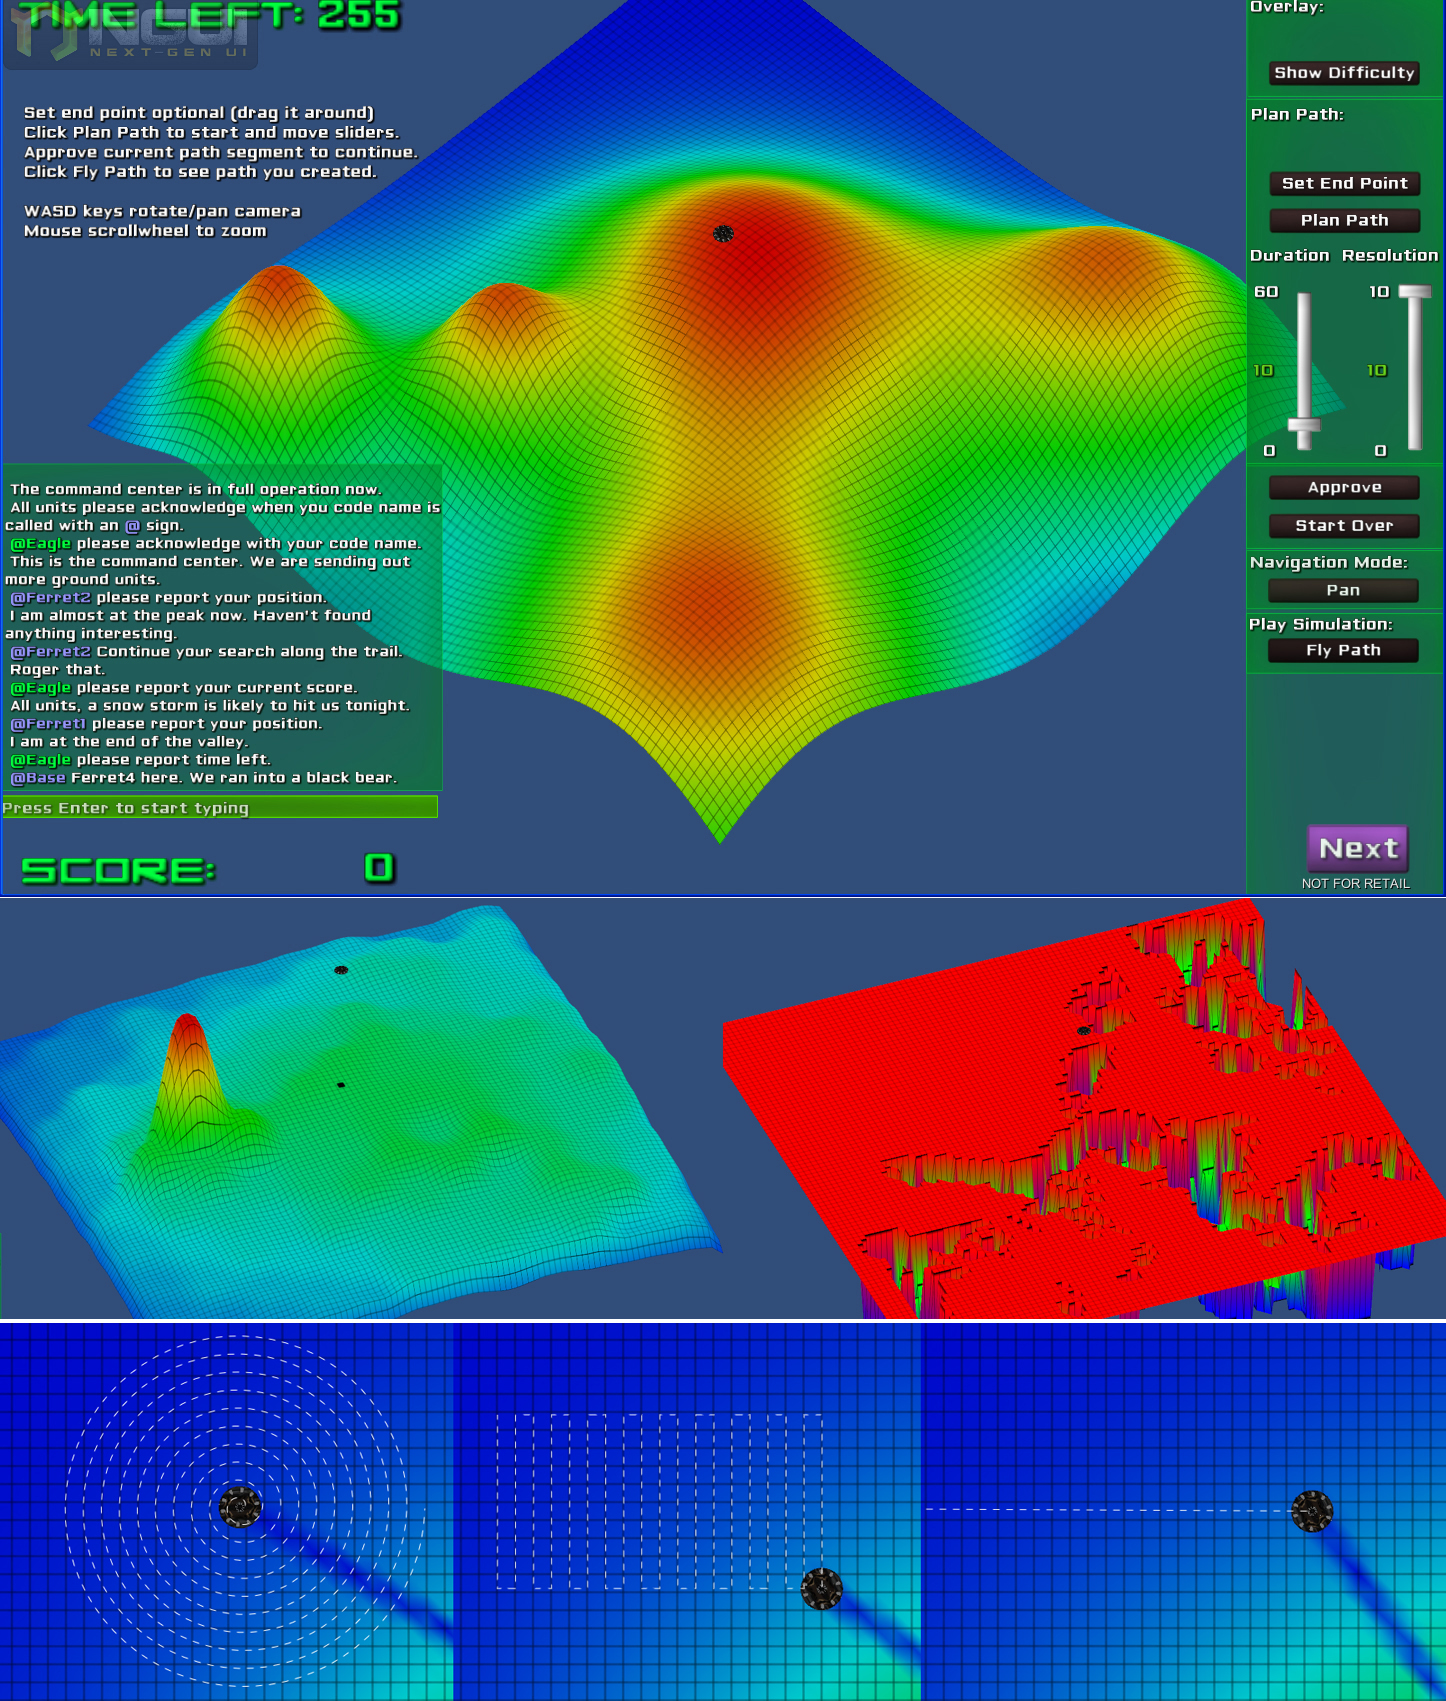
\includegraphics[width=3.5in]{UserStudy.JPG}
\caption{Top: User study simulation interface with sliding autonomy method showing the probability distribution map for scenario 1. Middle left: Probability distribution map for scenario 2. Middle Right: Task-difficulty map for scenario 2. Bottom: The three patterns available to user in pattern planning mode, spiral, lawnmower, and line.}
\label{UserStudy}
\end{figure}

We performed a 2$\times$3 within-subject design with 2 scenarios (easy vs difficult) and 3 planning methods (manual, pattern, and sliding autonomy). All participants completed all 6 exercises. We counterbalanced the order of the scenario and planning methods to reduce learning effect. Half of the participants started with scenario 1 (the other half scenario 2). and the order of the planning methods were randomly drawn without repeat from the permutation of all possible combinations (without following the same order in both scenarios).

%===================================================
\subsection{Participants}

After analyzing data collected from a pilot study with 6 volunteers, it was determined that 25 participants would likely produce significant test results. We recruited a total of 26 college students (14 male males and 12 females) between the age of 19 and 30 (average 22.89). None has colorblindness. The majority has no experience with robots (57.69\%), and 34.62\% of them are slightly experienced with vacuuming robots.

%===================================================
\subsection{Simulation Environment}

The user study is conducted in a 3D simulation environment. The top portion of Figure~\ref{UserStudy} shows a screen capture of the simulation interface. Both the probability distribution map and the task-difficulty map are displayed as 3D surfaces with a color map (red means high altitude and blue means low). The user can switch between the two maps anytime. The user can also rotate/pan a map and zoom in/out at will. The UAV in the simulation is a hexacopter that is capable of flying in all directions or hover in the same spot.

With the \textbf{manual} planning method, the user can fly the UAV around with arrow keys as the clock runs in a sped up fashion. The user can freely switch between two flying modes, turn mode and strafe mode, and four camera views, global view (always north up with full view of the map), behind view, bird's eye, and free form view (where the user can rotate/pan/zoom while flying). The user can pause/resume the flight and path planning to perform the secondary task or just review the search area for better planning.

With the \textbf{pattern} planning method, the user can choose from three simple patterns (spiral, lawnmower, and line as shown in the bottom portion of Figure~\ref{UserStudy}) and join these patterns to form the final path. As the user moves the cursor around, the size of the pattern changes with the cursor position marking the end of the path segment (up to the remaining flight time to keep the path valid). Rotation of the lawnmower pattern can be achieved by rotating the map left/right instead. And rotating the map up/down turns the perfect spiral pattern into an ellipse pattern. The user also can undo the last path segment created all the way back to the start. This planning method is ``semi-autonomous'' because the patterns are generated automatically without manually setting waypoints.

With the \textbf{sliding autonomy} method (top portion of Figure~\ref{UserStudy}), the user can (optionally) set an end point anywhere on the map (reachable within remaining flight time) for the current path segment and then see the path suggested by autonomy. Then he/she can drag the knob of the left slider to change the amount of time allocated to autonomy, and see path suggested by autonomy instantly for each time allocation as the knob of the slider is dragged up or down. The slider's max value always reflects the remaining flight time (in minute) for the user to plan. If the user is happy with the current path segment, he/she approves it, the UAV moves to the end of the path segment, and the process repeats until all flight time has been planned. The path planning algorithm used in this planning method is the LHC-GW-CONV algorithm described in~\cite{Lin2009UAV, Lin2014Hierarchical}. We choose this algorithm because it is the fastest algorithm.

The right slider is used to set the resolution or step value of the left slider and has a range between 1 and 10. For example, if the value of the right slider is set to 10, moving the left slider from bottom up will change time allocation to 10, 20, 30, ..., respectively. The purpose of the second slider is to improve the interaction experience when the user moves the left slider, because in order to provide instant feedback, paths with different time allocation need to be pre-computed by autonomy. Although each path only takes a fraction of a second to generate, for a 60-minute flight autonomy has to generate 60 paths for all possible time allocations, which can take a long time. When the value of the second slider is set high, only a small number of paths need to be pre-computed which enables the instant feedback. This feature turned out to have negative effect on users' interaction experience, which we will discuss later.

With all three planning methods, the user can choose to start over at any time during the exercise, and can restart as many time as exercise time allows, and we record the best path out of all tries. Each user fully understands how the manual and pattern planning methods work, but does not know how path planning autonomy generates paths behind the scene in the sliding autonomy method.

%===================================================
\subsection{Scenarios}

The user study contains two WiSAR scenarios. Scenario 1 is a synthetic case with a probability distribution map that is a mixture of five Gaussians (shown in the top portion of Figure~\ref{UserStudy}). No task-difficulty map is used in this scenario (uniform detection probability is assumed). 

Scenario 2 comes from a real WiSAR scenario, in which An elderly couple was reported missing near the Grayson Highlands State Park in Virginia. The probability distribution map used for this scenario (Figure~\ref{UserStudy} middle left) was generated using a Bayesian model~\cite{Lin2010Bayesian}. The map has been evaluated at George Mason University's MapScore web portal~\cite{Twardy2012MapScore} and performed better than most other models evaluated\footnote{Scoring 0.8184 on a [-1,1] scale where the higher the score the better. http://sarbayes.org/projects/}. This scenario also uses a task-difficulty map, and the map (Figure~\ref{UserStudy} middle right) was generated using vegetation density data downloaded from the USGS web site and categorized into three difficulty levels (sparse, medium, and dense, with detection probability of 100\%, 66.67\%, and 33.33\% respectively).

Scenario 2 is clearly more complicated than scenario 1 because the user also has to consider the different detection probability defined by the task-difficulty map. We refer to scenario 2 as the high information scenario and scenario 1 as the low information scenario.

%===================================================
\subsection{Secondary Task}

In each exercise, we also ask each participant to perform a secondary task together with the main task of path planning. This way we can measure the mental workload of the user. The secondary task is in the form of a group chat window (see the lower left corner of the top picture in Figure~\ref{UserStudy}), and when the user's code name ``Eagle'' is called, the user is asked to answer simple questions by typing in the chat window. Every 3 seconds (plus a random integer drawn from the uniform distribution [-2,2]) a text message is sent to the chat window, and every 5th message asks the user a simple question. Therefore, every minute the user receives 20 messages and 4 of them are directed to the user. For the same scenario and the same planning method, all users use the same set of chat messages.

We choose to use a group chat window as the secondary task because this is typical in real SAR operations. We also designed the chat messages to simulate a real WiSAR search. The user is asked to acknowledge connection and report path planning status periodically. This design ensures that the secondary task is ecologically valid~\cite{Vicente1997Should,Rasmussen1994Cognitive} and makes the experiment result more convincing.

%===================================================
\subsection{Procedure}

Each participant first fills out a demographic survey after signing the IRB consent form, then he/she completes four training exercises. The first three training exercises teach the user how to plan paths with the three planning methods using a simple probability distribution map and no task-difficulty map. The fourth training exercises adds the task-probability map to the path planning problem, and the user gets to practice the manual planning method again. Each training exercise lasts 5 minutes and the user cannot skip it. A ``cheat sheet'' is provided to each participant during the entire user study to explain the simulation environment and key concepts. Each participant is also asked to read the instructions for the NASA TLX survey.

Then each participant completes the six exercises (2 scenarios and 3 planning methods each) in a counterbalanced order. For each exercise the user has up to 5 minutes to plan a path. Once the user is happy with the path generated, he/she can finish the exercise early. We choose this design because we do not want the user to put all effort into completing the secondary task once he/she considers the primary task completed, which would skew the measurements on secondary task performance.

After the user completes each exercise, we ask the user to complete a NASA TLX survey for the exercise. Then after all six exercises are completed, the user fills out a post user study survey describing his/her subjective preference with the three planning methods.

%===================================================
\subsection{Measures}

We use the following five measurements for the primary path planning task:

\begin{itemize}
\item \textbf{Percent score}: In each exercise, an exercise score is computed by summing the amount of probability collected by the UAV if it followed the path planned. The user's best score for each exercise (because the user can have multiple tries) is normalized by dividing the best score from all users for the same scenario to compute the percent score. This way we can compare planning methods across scenarios.
\item \textbf{Time spent}: How much time is spent with each exercise.
\item \textbf{Try count}: How many times the user tried in each exercise. Note that because the manual planning method takes much longer time to plan a path than the other two methods by design, this measurement is used mainly to compare between the pattern and sliding autonomy planning methods.
\item \textbf{Mouse clicks per try}: How many times the user left-clicked the mouse within a try. Again, this measurement is used to compare pattern and sliding autonomy planning methods because manual planning methods does not require a lot of mouse clicks by design.
\item \textbf{NASA-TLX raw score}: The sum of user subjective evaluation of cognitive workload in six dimensions normalized to a 100-point scale. 
\end{itemize}

The following two measurements are used for the secondary task:
\begin{itemize}
\item \textbf{Percent of questions missed}: What percentage of questions directed to the user were missed before user completed the exercise. Here we do not measure the percent of questions answered correctly because all the questions are very simple and all users answered the questions correctly.
\item \textbf{Chat latency}: The number of seconds between the time a question was presented to the user and the time when the user answered the question.
\end{itemize}

%=================================================================================	
\section{Results and Analysis} 
\label{sec:Results}

We analyzed data recorded with a repeated measure ANOVA and report results in this section.

%===================================================
\subsection{Compare Across Scenarios}

During the user study, each participant worked through two WiSAR scenarios. In scenario 1 (low information) no task-difficulty map is used. In scenario 2 (high information) because partial detection is enforced, the amount of probability that can be collected (exercise score) in scenario 2 is much lower than in scenario 1. In order to show a fair comparison across scenarios, we use percent score instead, which is a percent comparing the participant's score to the best performing participant's score in the same scenario.

Table~\ref{AcrossScenarios} lists the user study results compared between scenario 1 and 2 with statistically significant results highlighted in bold. Average participant percent score is very close in both scenarios because we normalized exercise scores. So an average participant's performance against the highest score is about 75\% in each scenario. There is a slight difference of 26 seconds in average time spent, which is not significant compared to the 300 seconds given for each exercise. Average try count in both scenarios are close enough, meaning each participant had enough time in each exercise to give each scenario a few tries.

Mouse clicks per try for the two scenarios are significantly different ($F=$ 28.65, $p<$ .0001) indicating scenario 2 required more physical work from each participant than scenario 1. This result matches the difficulty of the two scenarios where each participant created more path segments with the pattern and sliding autonomy planning methods in scenario 2 because it uses a task-difficulty map with many ``valleys''.

NASA TLX score is also significantly different ($F=$ 31.35, $p<$ .0001) between the two scenarios where the average score difference is 9.98 (out of a total of 100 points), almost a full ``pip'' on the TLX survey, indicating that on average each participant felt his/her cognitive workload was much higher in the high information scenario.

The percent of questions missed is only slightly different between scenarios (52.94\% and 56.69\%), and the chat latency is also very close (10.39 and 11.17 seconds). This shows that participants performed about the same on average with the secondary task across scenarios.

If we only look at the performance of the sliding autonomy planning method across scenarios, results follow the same trend. Therefore we do not list the results separately.

\begin{table}
\caption{Comparing across scenarios}
%\small
\scriptsize
	\centering
		\begin{tabular}
			{|l|c|c|c|c|}
			\hline
			& S1 Low & S2 High & SE & Significance \\
			\hline
			Score \% & 76.99 & 74.17 & 1.12 & $F$=7.51, $p$=.0112 \\
%			\hline
			Time spent & 224.01 & 250.47 & 12.06 & $F$=8.35, $p$=.0079 \\
%			\hline			
			Try count & 3.08 & 2.67 & 0.37 & $F$=3.32, $p$=.804 \\
%			\hline			
			Clicks/try	& 15.95 & 33.54 & 2.59 & \textbf{$F$=28.65, $p<$.0001} \\ 
%			\hline
			NASA TLX & 48.19 & 58.17 & 2.50 & \textbf{$F$=31.35, $p<$.0001} \\ 
			\hline
			Q. missed \% & 54.88 & 54.90 & 5.18 & $F$=0.00, $p$=.9941 \\ 
%			\hline
			Chat latency & 10.88 & 10.77 & 0.56 & $F$=0.03, $p$=.8755 \\ 
			\hline			
		\end{tabular}
%\vspace*{2ex}
%\vspace*{-2ex}
\label{AcrossScenarios}
\end{table}

%===================================================
\subsection{Compare Across Planning Methods}

For each scenario, three path planning methods were used. Table~\ref{AcrossMethods} lists comparison among the three methods. 

The performance difference in percent score is statistically significant ($F=$ 223.03, $p<$ .0001) with pattern (72.75\%) performing better than manual (59.40\%) and sliding autonomy (94.60\%) performing better than pattern. As shown in Figure~\ref{PerformanceDifference}, this trend is also clear in both scenario 1 and 2. Therefore, user study results show strong support for our first hypothesis: sliding autonomy method performs better than either the manual method or the pattern method in both low information and high information scenarios.

\begin{table}
\caption{Comparing across planning methods}
%\small
\scriptsize
	\centering
		\begin{tabular}
			{|l|c|c|c|c|c|}
			\hline
			& M & P & SA & SE & Significance \\
			\hline
			Score \% & 59.40 & 72.75 & 94.60 & 1.39 & \textbf{$F$=223.03, $p<$.0001} \\
%			\hline
			Time spent & 243.35 & 240.02 & 228.37 & 12.06 & $F$=1.16, $p$=.3226 \\
%			\hline			
			Try count & 1.75 & 3.56 & 3.31 & 0.43 & $F$=9.47, $p$=.0003 \\
%			\hline			
			Clicks/try & 13.01 & 35.64 & 25.58 & 2.90 & \textbf{$F$=19.47, $p<$.0001} \\
%			\hline
			NASA TLX & 61.51 & 49.18 & 48.86 & 2.81 & \textbf{$F$=14.15, $p<$.0001} \\
			\hline
			Q. missed \% & 52.94 & 56.69 & 55.04 & 5.17 & $F$=1.26, $p$=.2915 \\
%			\hline
			Chat latency & 10.39 & 11.17 & 10.92 & 0.65 & $F$=0.46, $p$=.6327 \\
			\hline			
		\end{tabular}
%\vspace*{2ex}
%\vspace*{-2ex}
\label{AcrossMethods}
\end{table}

\begin{figure}
\centering
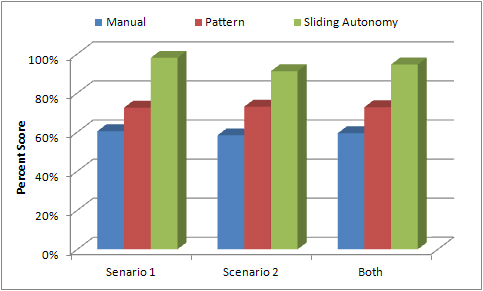
\includegraphics[width=3.5in]{PerformanceDifference.JPG}
\caption{Performance difference for three path planning methods.}
\label{PerformanceDifference}
\end{figure}

Statistically significant difference was also found in mouse clicks per try ($F=$19.47, $p<$.0001). The manual method uses arrow keys to fly the UAV around and only uses mouse clicks when switching camera modes or stop the timer in order to perform the secondary task. Therefore, by design, this method does not use a lot of mouse clicks. Pattern and sliding autonomy methods both use mouse clicks for the actual path planning task, and the pattern method clearly generated more mouse clicks per try (35.64) than the sliding autonomy method (25.58). Two factors might have contributed to this difference, first one being that the pattern method allows undoes while the sliding autonomy method does not support this function. Also with the sliding autonomy method a participant can drag the slider and see different suggestions from path planning autonomy, which does not require a lot of mouse clicks.

NASA TLX raw scores show significant differences among the three methods ($F=$14.15, $p<$.0001), with the manual method showing the highest cognitive mental workload (61.51), a full ``pip'' more than the other two methods. However, the score difference between the pattern method and the sliding autonomy method is small. Figure~\ref{NASATLX} shows the box plots of the NASA TLX scores for each scenario. Participants felt that the pattern method and the sliding autonomy method required about the same amount of cognitive mental workload in each scenario, and the manual method required a lot more mental workload in both scenarios.

\begin{figure}
\centering
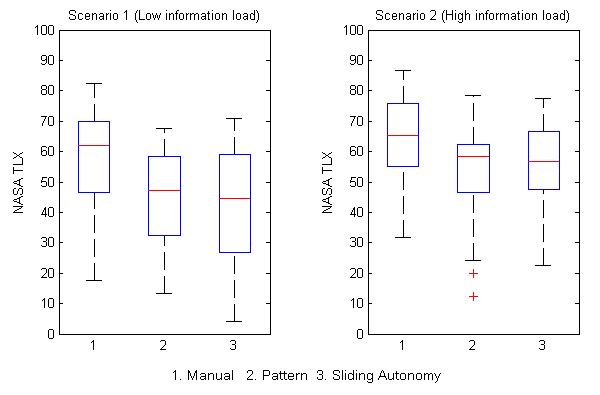
\includegraphics[width=3.5in]{NASATLXBoxPlot.JPG}
\caption{Box plots of the NASA TLX scores for each scenario.}
\label{NASATLX}
\end{figure}

For all three planning methods, participants performed about the same on the secondary task, as shown by percent of questions missed and chat latency in Table~\ref{AcrossMethods}. Combining this with percent score and NASA TLX we can conclude that sliding autonomy performed best without increasing participants' mental workload, which support our third hypothesis: Sliding autonomy method does not increase the mental workload of the operator when compared against manual and pattern methods.

If a participant allocates the entire flight time (60 minutes) to path planning autonomy (LHC-GW-CONV algorithm), the path is generated by full autonomy without any human input. The percent score for this path would be 96.13\% for scenario 1 and 78.83\% for scenario 2. This is better than the average performance of the manual and pattern methods in both scenarios as shown in Figure~\ref{PerformanceMarkers}. If we compare each person's percent score against full autonomy out of all 26 participants, in scenario 1, none could outperform full autonomy using the manual and pattern methods, but 23 (88.46\%) were able to perform better with sliding autonomy (human-autonomy team). In scenario 2, no one did better using the manual method, 5 (19.23\%) did outperform full autonomy using the pattern method, and 24 (92.31\%) were able to beat full autonomy using the sliding autonomy method. Table~\ref{CompareToFullAutonomy} summarizes the comparison. User study results clearly show that the human inputs made significant differences and human-autonomy team outperformed autonomy working alone. This also strongly supports our second hypothesis: Sliding autonomy method performs better than autonomy working alone in both low information and high information scenarios.

\begin{figure}
\centering
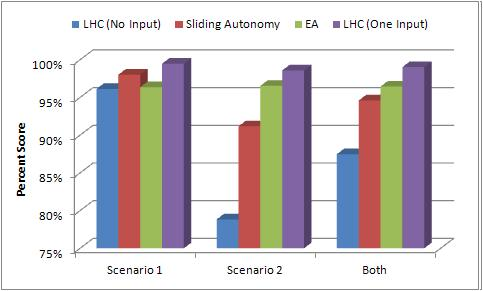
\includegraphics[width=3.5in]{PerformanceMarkers.JPG}
\caption{Comparing sliding autonomy performance against various markers.}
\label{PerformanceMarkers}
\end{figure}

\begin{table}
\caption{Percent of participants outperforming autonomy with each method}
%\small
	\centering
		\begin{tabular}
			{|l|c|c|c|}
			\hline
			 & Manual & Pattern & Sliding Autonomy \\
			\hline
			Scenario 1 (Low) & 0\% & 0\% & \textbf{88.46\%} \\
			\hline
			Scenario 2 (High) & 0\% & 19.23\% & \textbf{92.31\%} \\
			\hline			
		\end{tabular}
%\vspace*{-2ex}
\label{CompareToFullAutonomy}
\end{table}

%===================================================
\subsection{Additional Factors}

We also performed ANOVA analysis on some additional factors that might create differences: gender, experience in video games, order of the scenarios, and whether participants used full autonomy with the sliding autonomy method. No significant differences were found for these factors overall, across scenarios, or across methods. Table~\ref{OtherFactors} below lists analysis results. There is also no significant correlation (-0.2259) between percent of questions missed in the secondary task and the NASA TLX raw scores.

\begin{table}
\caption{ANOVA Analysis Results for Additional Factors}
%\small
\scriptsize
	\centering
		\begin{tabular}
			{|l|c|c|c|}
			\hline
			 & Overall & Scenario & Method \\
			\hline
			Gender & $F$=0.05, $p$=.8292 & $F$=0.76, $p$=.3930 & $F$=0.59, $p$=.5602 \\
			\hline
			Video Game Exp. & $F$=0.78, $p$=.5497 & $F$=1.64, $p$=.2011 & $F$=1.13, $p$=.3650 \\
			\hline
			Scenario Order & $F$=0.09, $p$=.7672 & $F$=0.39, $p$=.5378 & $F$=1.53, $p$=.2278 \\
			\hline
			Full Autonomy & $F$=3.70, $p$=.0675 & $F$=0.36, $p$=.5559 & $F$=0.04, $p$=.9599 \\
			\hline			
		\end{tabular}
%\vspace*{-2ex}
\label{OtherFactors}
\end{table}

%=================================================================================	
\section{Discussion} 
\label{sec:Discussion}

%===================================================
\subsection{Planning methods looking more closely}

With the manual method, the user uses arrow keys to move the UAV around to create a path, so by design the method is very intuitive, flexible, and requires more physical interactions (keyboard, not mouse clicks). But in order to plan a 60-minute path in 2 minutes, the UAV has to move very quickly in the simulation environment. We made sure each user can complete at least two tries using this method while performing the secondary task simultaneously. High UAV speed makes it harder to navigate accurately. Many participants called the arrow keys too ``sensitive'' and recommended slowing down the UAV. Because of the time pressure, the path planning task is more of a continuous process. Therefore, when errors are made, it is too costly to start over (we did not provide an undo function). The user also does not have the luxury to pause the planning in order to think through strategies in his/her head; it has to be done while the user is moving the UAV around. Naturally, when this continuous process is frequently interrupted by the secondary task where the user has to pause planning and answer questions in the group chat window, user frustration goes high. More physical work, higher frustration, and low performance score are the main factors contributing to a much higher NASA TLX score for the manual method. Although this planning method supports four camera views and two flying modes, most participants chose to stick with free form view where the entire search region is displayed and with strafe mode to avoid getting confused with UAV orientation. During training, participants actually had one extra exercise with the manual method, but this method still performed the worst.

With the pattern method, the user joins a mixture of three patterns (spiral, lawnmower, and line) together to form the final path. This is more of an episodic process, so it is very easy to pause in the middle of the planning and shift attention to the secondary task. There is also less time pressure because the user can quickly plan for the remaining time with just one big spiral (or lawnmower) in one click. Therefore, the user has plenty of time to try many times with different strategies. In the post user study survey, many participants commented that with the spiral and lawnmower pattern it is really easy to run out of time. They suggested adding the ability to allocate time to the patterns similar to the sliding autonomy method. This means that with this method, a user enjoys the systematic coverage of an area but has a hard time estimating how much time it takes the UAV to cover the area following the pattern. Several participants also suggested adding more patterns to the method. The pattern method is the only method supporting undoes. This ability surely had impacts on number of mouse clicks per try and participants' preference over the three planning methods. Another interesting observation is that participants seemed to be overly optimistic about their performance using the pattern method. For example, although sliding autonomy performed better than pattern in all scenarios for all participants, in 46.15\% of the times, participants rated pattern as performing better than sliding autonomy in NASA TLX scores; and also in the post user study survey, 26.92\% participants (not the majority, but over a quarter of the population) actually believed the pattern method creates best paths.

Similar to the pattern method, the sliding autonomy method is also an episodic process. Therefore, stopping in the middle of the planning to answer questions for the secondary task was easy. And it only takes a few clicks to let full autonomy plan path for the remaining time, so there is not much time pressure and the user can have many tries. Because the user does not know how autonomy works behind the scene, many participants were surprised by the path recommended by autonomy, and feel that autonomy did not do what they had tell it to do. For example, when a user sets the end point in region A, autonomy might plan a path that spends most of time in a seemingly unrelated region B and only goes toward region B at the end of the path, because such a path is more efficient (scores higher). In such cases, the slider becomes the only tool that lets the user ``force'' autonomy to do what the user wants, and path planning turns into a fight between the user and autonomy. However, the instant feedback (displaying path and the predicted ``vacuuming effect'') does help the user figure out why autonomy would suggest something different, and some participants were glad that autonomy suggested better paths they had not considered. Most participants were generally happy with the path segment recommended by autonomy covering a local region, even when the region is in an irregular shape (not a circle or rectangle). Many participants also expressed that they did not have enough control over the path generation and recommended adding the ability to include constraints such as ``middle points'' where the path segment has to go through these middle points. In fact, such ``middle points'' can already be achieved with the current method by setting end points. Several participants complained that this method does not have the undo function. They also wanted the ability to see how suggested path changes when the end point is moved around, which is an idea worth exploring because it allows the user to not only slide along the time allocation dimension, but also slide along the constraints dimension and see instant feedback. With both the pattern and sliding autonomy methods, many participants expressed the desire to be able to modify the path after it is generated.

In scenario 2 where a task-difficulty map was used, because the probability map is similar to a unimodal distribution (see middle portion of Figure~\ref{UserStudy}, most participants chose to first cover the probability hill use the probability distribution map, and then planned the remaining path using only the task-difficulty map view in all three methods. If the probability distribution map is more complex with many probability hills, then likely the user will be switching between the two maps back and forth in order to incorporate information. Some suggested showing both maps side by side or have a way to combine the two maps into one. These ideas are worth exploring in future user studies.

In the post user study survey, the majority of the participants think manual is the easiest to learn (53.85\%), pattern is the easiest to use (57.69\%), and sliding autonomy performed the best (65.38\%). However, most participants preferred the pattern method (69.23\%) out of all three. We believe the inability to undo, not able to move the end point once path is suggested, and the second slider in the interface (which we will discuss in a later section) all had negetive impacts on participants' preference over the sliding autonomy method. Once these functions are in place, the sliding autonomy method will become more preferrable than the pattern method.

%===================================================
\subsection{Trust in autonomy}

The algorithm we used for the sliding autonomy method is the LHC-GW-CONV algorithm. We selected this algorithm because of its fast speed. If speed is not a concern, then the Evolution Algorithm (EA) we developed~\cite{Lin2009UAV} can autonomously generate even better paths. For example, the percent score for EA would be 96.36\% for scenario 1 and 96.54\% for scenario 2. In scenario 1, the score is only slighly better than full autonomy in sliding autonomy (96.13\%), but in scenario 2, the score is much better than full autonomy (78.83\%). We also used the sliding autononomy method and generated paths for both scenario 1 and 2 with only one human input, an end point. Using the best score out of 3 tries (roughly equal to the average number of tries in the user study), we also computed the percent score for this autonomy+1 human input approach: 99.47\% for scenario 1 and 98.58\% for scenario 2. Using the EA and Autonomy+1 score as additional markers, we plotted participants average performance in each scenario against these markers. Figure~\ref{PerformanceMarkers} shows the result.

First, sliding autonomy (human-autonomy team) outperformed autonomy (LHC-GW-CONV algorithm) in both scenarios. Sliding autonomy also outperformed EA in scenario 1 (low information). In scenario 2, the performance of sliding autonomy is not very far from EA (5.36\%), and the difference is even smaller (1.85\%) when averaged over both scenarios. However, the most interesting observation is that autonomy+1 actually outperformed all others in both scenarios (99.47\% for scenario 1 and 98.58\% for scenario 2). Although a few participants did score higher than autonomy+1, the difference is less than 1.5\%. Table~\ref{CompareToMarkers} lists what percentage of participants outperformed full autonomy, EA, and autonomy+1.

What Figure~\ref{PerformanceMarkers} suggests is that with the sliding autonomy method, it does not need a lot of human inputs to perform really well. Instead of spending the effort creating many path segments and set many end points, it is probably more rewarding to search for the right region to set just one or two constraints. However, 88.68\% of participants gave more than 1 input when they used sliding autonomy (81.13\% for 2 inputs and 69.81\% for 3 inputs). This suggests that human users lacked trust for the performance of autonomy. In the post user study survey, only 46.15\% participants acknowledged that he/she used full autonomy during path planning with the sliding autonomy method. This number also indicates that most participants did not trust autonomy. When using the sliding autonomy method, a good strategy is actually to start with full autonomy (as the worst performance base) and then see how additional human inputs can improve the path.

%Moray~\cite{Moray1999Mental} provides a good summary of how mental models are used and proposes that mental models ``allow operators to think about causal structures and functions in systems which they must control....'' Goodrich and Boer present a case study of Adaptive Cruise Control design and explain how an automobile driver can switch among multiple mental models and use different management strategies~\cite{Goodrich2002Multiple, Goodrich2003Model}. 

Lee and See propose that because people respond to technology socially, trust guides reliance when unanticipated situations make it impractical or impossible to understand automation~\cite{Lee2004Trust}, and defined \textit{distrust}, ``trust falls short of the automation's capabilities'', and \textit{overtrust}, ``trust exceeds system capabilities''. Bradshaw et al.\ \cite{Bradshaw2013Seven} had similar definitions and used the term \textit{under-reliance} for distrust, instead. Both suggested that trust in automation should be ``calibrated''. Hoffman et al.\ \cite{Hoffman2013Trust} suggests ``active exploration for trusting''(AET) and hope this approach can promote both trust ``calibration'' and appropriate reliance. We believe the sliding autonomy approach we propose can also be used for trust calibration. As the user is dragging the knob on the slider, he/she is calibrating his/her trust on path planning autonomy. In our user study, all participants only had 30 minutes of training before using the sliding autonomy method. We speculate that as the user gets more familiar with the sliding autonomy approach in the long run, he/she would be able to calibrate trust better. However, validation of this claim is beyond the scope of this paper and will be part of a future long-term user study.

When more complicated probability distribution map and task-difficulty map are used, it is possible that the human user will see more value in the sliding autonomy approach because combining this much information in human mind and then decide trade offs in path planning required much more computation. And when the human user finds himself/herself incapable of such tasks, he/she might rely on autonomy to help solve the puzzle, and the sliding autonomy approach becomes more useful in calibrating trust. Validating this hypothesis is another natural extension of the present work.

\begin{table}
\caption{Percent of participants outperforming autonomy performance markers}
%\small
	\centering
		\begin{tabular}
			{|l|c|c|c|}
			\hline
			 & Autonomy & EA & Autonomy+1 \\
			\hline
			Scenario 1 (Low) & \textbf{88.46\%} & \textbf{88.46\%} & 7.69\% \\
			\hline
			Scenario 2 (High) & \textbf{92.31\%} & 26.92\% & 15.38\% \\
			\hline			
		\end{tabular}
\label{CompareToMarkers}
%\vspace*{-2ex}
\end{table}

%===================================================
\subsection{Why human-autonomy team performs better?}

User study results show that the human-autonomy team outperformed either human or autonomy working along. But how were they able to achieve this? We believe that the reason is: the sliding autonomy approach enabled the human to focus on what human is good at and autonomy to focus on what autonomy is good at. Bradshaw et al.\ pointed out in~\cite{Bradshaw2013Seven}: ``Humans, though fallible, are functionally rich in reasoning strategies and their powers of observation, learning, and sensitivity to context.'' Our observation suggests that human is really good on two things: planning strategically and recognize bad path segments.

The sliding autonomy method lets the user plan at a higher abstract level by specifying priorities in search sub-regions and how well each sub-region should be covered. Then how to cover the sub-region well given a fixed flight time is left for autonomy to handle. Autonomy, on the other hand can generate a path that covers a sub-region (or some nearby sub-regions) precisely and quickly, and can handle all kinds of irregular sub-region shapes. Therefore, the sliding autonomy method combines the strengths of both human and autonomy.

A human user is also very good at recognizing bad moves in solutions suggested by autonomy. The sliding autonomy approach enables the human user to select from a bunch of suggested paths, selecting a path segment with fewer bad moves (which might not actually be bad in autonomy's perspective with just the current path segment) will probably increase the chance of a good final path. So again, the sliding approach takes advantage of the strengths of both human and autonomy.

%===================================================
\subsection{Why similar secondary task performance in all three methods?}

The pattern and sliding autonomy methods are episodic, suggesting that it is easier for the user to pause planning and shift attention to the secondary task of answering questions in the group chat window. It almost seems a natural conclusion that the user should have performed better with the secondary task compared to the manual method. However, user study data shows that there is no significant differences in the users secondary task performance across all three path planning methods.

The manual method required a lot of continuous keyboard interaction (great physical demand and temporal demand) to move the UAV around. However, it does not actually require a lot of mental demand and effort because in the user's mind he/she is not actually planning things in great detail. If a mistake is made in the path planning, because there is no way to correct it, the user quickly drops it out of his/her mind and stop worrying about it. The planning process is more sporadic and spontaneous. Therefore, the low mental demand and effort makes monitoring the group chat window an easy task, even though switching back between primary task and secondary task is very frustrating.

With the pattern and sliding autonomy methods, path planning is more like piecing together a puzzle. The user is deeply drawn into the problem solving mode, and has to consider many trade offs in his/her mind, which actually required more mental involvement. With the sliding autonomy method, the user is interacting with complicated algorithms, so while planning a path, the user is also trying to build a mental model of how autonomy works. Therefore, the user actually paid less attention to the secondary task. Fighting with autonomy when human and autonomy had disagreements and the user's struggle with the second slider also drew user attention away from the group chat window. But when the group chat window catches the user's attention, he/she can perform the secondary task leisurely.

Another factor affecting the secondary task performance is summarized by David Woods and Eric Hollnagel as the law of stretched systems~\cite{Woods2006Joint}: ''every system is stretched to operate at its capacity; as soon as there is some improvement, for example in the form of new technology, it will be exploited to achieve a new intensity and tempo of activity.'' Therefore, with the pattern and sliding autonomy methods, people had more tries and evaluated more options and trade offs. With the sliding autonomy method, this means the user played with more time allocations and evaluated more paths suggested by path planning autonomy, which ultimately resulted in better quality paths at the cost of not so great performance in the secondary task.

%===================================================
\subsection{Fighting with Human Nature}

It seems buried deeply in human nature that when a user performs an action, he/she wants immediate feedback so badly that when no such feedback is available, he/she cannot fight the urge to perform more actions thinking the additional actions would generate some feedback. To meet this demand, when we designed the sliding autonomy interface, we implemented two sliders where the second slider sets the step size value of the first slider. We had hoped that this would reduce the number of paths we had to pre-compute and make the user experience smoother by providing instant path feedback when they move the first slider. Observations from the user study show that this design actually negatively affected the user experience and increased user's cognitive workload. Which also means a better design with this element could potentially improve the user's performance and preference with the sliding autonomy method.

Because when the value of the second slider is changed, the value of the first slider is also changed to reflect the smallest number that is a multiple of the selected step value. This behavior created multiple problems. First, some users quickly learned that changing the value of the second slider also changes time allocation to the path planning task, and started using this slider to set time allocation instead. This meant that more paths actually had to be pre-computed behind the scene, and in the user's eyes now the system was no longer providing instant feedback. So he/she began moving the slider randomly with the hope to generate some feedback, which meant more paths had to be pre-computed. A very bad cycle. Secondly, even though during training each user is told that there might be slight delay when they move the main slider in some cases, in the real exercises, they still wanted instant feedback. And when instant feedback was not available, they fell in the trap of operator-induced oscillation, and had to make several tries to set the value they desire. Fighting with the sliders required additional attention, so less attention were paid to monitor the group chat window. A ``please wait'' message would probably have less negative impact on the user's experience.

When a human sees an ``obvious error'' in a path segment, the urge to correct is typically so strong that it draws all the attention to the quest, turning the path planning task into a fight with autonomy at the cost of increased cognitive workload. The ``obvious error'' could mean two different cases. In the first case, the ``error'' is indeed a bad move that can be easily modified in the user's mind to improve the path performance. In the second case, the ``error'' is actually not a bad move, only that the user cannot comprehend the reason behind the move, so there is still a strong desire to change it. However, because there is no direct way for the user to modify the path, the user can only change the path by moving the slider to set different time allocation, sometimes this ``error'' simply cannot be modified. The user wastes time trying, user's cognitive workload increases, and the user has a bad experience with the sliding autonomy method.

There are probably more things than what we discussed here that could have improved the user experience and improve the user's performance on both the primary task of path planning and the secondary task of answering questions in the group chat window. We just want to emphasize that even with these negative impacts, the sliding autonomy method still performed significantly better than the other two methods and autonomy working alone without increasing the user's mental workload.

%=================================================================================	
\section{Conclusions and Future Work} 
\label{sec:Conclusions6}

In this paper we propose a new autonomy management approach, sliding autonomy, which lets the user influence the behavior of the autonomous system along three new dimensions: information representation, task constraints, and time allocation. We extend the autonomy design guideline in our prior work by adding a new row for intelligence of collaborative agents (including human-autonomy team), and explain how the three new dimensions fit into the guideline when we apply the proposed approach to the task of UAV (Unmanned Aerial Vehicle) path planning to support Wilderness Search and Rescue (WiSAR). Experiment results from a user study validate our hypotheses and show that the sliding autonomy method performs significantly better than either the manual or pattern path planning method without increasing the user's mental workload, and the human-autonomy team outperforms either human or autonomy working alone.

Possible future work include evaluating the sliding autonomy approach in a long-term study and see how the user's trust can be calibrated. More complicated WiSAR scenarios can be tested and see how that affects the human-autonomy interaction and the performance of the human-autonomy team. Another user study can evaluate how well the human-autonomy team can work with outdated information representation using the sliding autonomy approach. It would also be interesting to investigate the human-autonomy interaction experience when the ability to modify information representation is added to the tool.

%=================================================================================	
\section*{Acknowledgments}

This work was partially supported by 
the National Science Foundation 
%\_\_\_\_\
under grant number 
0534736 
%\_\_\_\_\_
and by a grant from
the Army Research Laboratory.
%\_\_\_\_\.
Any opinions, findings, and conclusions or recommendations expressed in this material are those of the authors and do not necessarily reflect the views of the sponsoring organizations.

%% Use plainnat to work nicely with natbib. 

\bibliographystyle{IEEEtran}
\bibliography{LannyDissertation}

%Properly evaluate human-robot interaction has always been a challenging problem due to the diversity of team setups, environmental contexts, and tasks involved. Many metrics have been proposed in the literature. Crandall and Goodrich proposed a metric called Neglect Time to measure interaction efficiency~\cite{Crandall2002Principles}. Together with Neglect Time, Olsen and Goodrich later added Task Effectiveness, Robot Attention Demand, Fan Out, and Interaction Effort to the list of Metrics~\cite{Olsen2003Metrics}. Steinfeld and et al.\ suggest some common metrics for standardizing task-oriented human-robot interaction~\cite{Steinfeld2006Common}. In~\cite{Olsen2007Evaluating}, Olsen presents a set of criteria for evaluating new UI systems. Crandall and Cummings propose in~\cite{Crandall2007Ddentifying} a set of metric classes that can predict how many robots should be in the team and the system effectiveness for single-operator controlling multiple robots. We follow guidelines provided in these papers to validate our proposed solution.

%In order to intelligently plan paths for a UAV, it is necessary to understand missing person behaviors and generate a probability distribution of likely places to find the missing person. Many researchers analyzed past WiSAR cases in order to understand missing person behaviors~\cite{Setnicka1980Wilderness,Hill1998Lost,Syrotuck2000Analysis,Heth1998Characteristics,Koester2008Lost}.~\cite{Syrotuck2000Introduction} describes how to use mathematical models to calculate the probability of detection, probability of area and probability of success. He also describes an example search mission. Researchers also looked at systematically utilizing GIS (Geographic Information System) information for search and rescue applications~\cite{Ferguson2008GIS,Soylemez2006Utility}.

%Due to factors such as lighting conditions, dense vegetation, or human observer cognitive workload, even when sensor footprint covers the location of the missing person, probability of detection can be less than 1. In the 1950's, Koopman discussed the uncertainties in the act of detecting hostile submarines with radars and proposed a concept called the instantaneous probability of detection by one glimpse~\cite{Koopman1956Theory}. He presented simple search algorithms and demonstrated how search effort should be distributed given a prior probability distribution of the target and known law of detection when only a limited total amount of search effort (or time) is available~\cite{Koopman1957Theory}. Stone~\cite{Stone1975Theory} presents various search plans with partial detection models using Lagrange multipliers and maximization of Lagrangians in finding stationary target in very basic search problems when no false targets are present. Washburn~\cite{Washburn1981Search} discusses how to construct optimal search paths for different search problems. The author also developed detection models based on radar/sonar and expanded the fundamentals of search theory to include moving targets. More recent work includes~\cite{Niedfeldt2010integrated} where Niedfeldt et al.\ present a UAV path planning algorithm that utilizes probability of detection and maximizes the probability of identifying an object using a N-step lookahead method, and~\cite{Ryan2010particle} where Ryan and Hedrick developed a control formulation for a fixed-wing UAV that minimizes the entropy of an estimate distribution over a receding horizon for searching a moving target over a fixed time horizon. Stone et al.\ used posterior probability maps and successfully located the wreckage of Air France Flight 447~\cite{Stone2011Search}. Metrics such as Koopman's instantaneous probability of detection by one glimpse~\cite{Koopman1956Theory}, ``seeability'' proposed by Morse et al.\ \cite{Morse2010UAV}, and terrain and vegetation information obtained from USGS~\cite{Lin2010Bayesian} can be used to build a task-difficulty map representing probability of detection in different search subregions.

%The UAV technology is an intelligent system with the integration of many component autonomous algorithms and user interfaces. Integration at this level requires tremendous effort. Salas and Fiore~\shortcite{Salas2004Team} provide great insights on challenges across people and machines, and across time and space in distributed teams. Sycara and Lewis~\shortcite{Sycara2002Integrating} also asked the questions: 1) can a software agent perform the task? and 2) can the agent's assistance contribute toward team performance? Tso et al.\ ~\shortcite{Tso1999Multi} identified that integrating a UAV into the search task creates at least two roles: a pilot that controls the UAV and a sensor operator that analyzes the sensor outputs, and lessons from other search-related domains~\cite{Drury2003Awareness} show that multiple roles are required and these roles can be supported by autonomy algorithms and user interface technologies. These findings motivate and guide our research in developing UAV technology to support WiSAR operations.

\end{document}